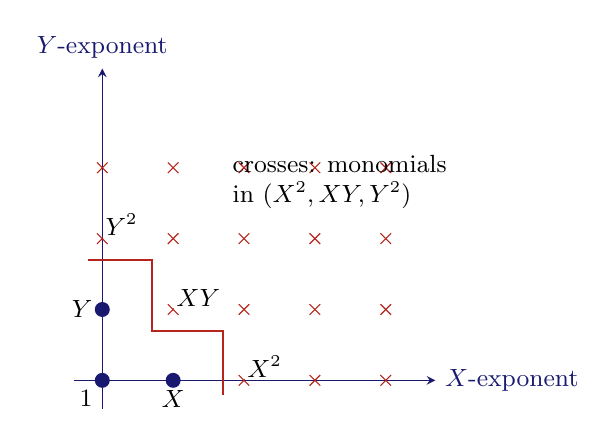
\begin{tikzpicture}[x=0.9cm,y=0.9cm,>=stealth,every node/.style={font=\small}]
\draw[->,MidnightBlue] (-0.4,0)--(4.7,0) node[right] {$X$-exponent};
\draw[->,MidnightBlue] (0,-0.4)--(0,4.4) node[above] {$Y$-exponent};
\foreach \i in {0,...,4} {
 \foreach \j in {0,...,3} {
  \pgfmathtruncatemacro{\d}{\i+\j}
  \ifnum\d>1
   \draw[BrickRed] (\i-0.075,\j-0.075)--(\i+0.075,\j+0.075);
   \draw[BrickRed] (\i-0.075,\j+0.075)--(\i+0.075,\j-0.075);
  \fi
 }
}
\fill[MidnightBlue] (0,0) circle (2.7pt);
\fill[MidnightBlue] (1,0) circle (2.7pt);
\fill[MidnightBlue] (0,1) circle (2.7pt);
\node[below left] at (0,0) {$1$};
\node[below] at (1,0) {$X$};
\node[left] at (0,1) {$Y$};
\draw[BrickRed,thick] (1.7,-0.2)--(1.7,0.7)--(0.7,0.7)--(0.7,1.7)--(-0.2,1.7);
\node[above right,fill=white,inner sep=1pt] at (2,0) {$X^2$};
\node[above right,fill=white,inner sep=1pt] at (1,1) {$XY$};
\node[above right,fill=white,inner sep=1pt] at (0,2) {$Y^2$};
\node[align=left] at (3.35,2.8) {crosses: monomials\\in $(X^2,XY,Y^2)$};
\end{tikzpicture}
